\documentclass[12pt,a4paper]{article}
\usepackage[utf8]{inputenc}
\usepackage{listings}
\usepackage{graphicx}
\usepackage{color}
\usepackage{xcolor}
\usepackage{caption}
\usepackage{subcaption}
\usepackage{hyperref}
\usepackage{tikz}
\usetikzlibrary{arrows,automata}

\definecolor{mygreen}{rgb}{0,0.6,0}
\definecolor{mygray}{rgb}{0.5,0.5,0.5}
\definecolor{mymauve}{rgb}{0.58,0,0.82}

\lstset{ %
  backgroundcolor=\color{blue!5},   % choose the background color; you must add \usepackage{color} or \usepackage{xcolor}
  basicstyle=\footnotesize,        % the size of the fonts that are used for the code
  breakatwhitespace=false,         % sets if automatic breaks should only happen at whitespace
  breaklines=true,                 % sets automatic line breaking
  captionpos=b,                    % sets the caption-position to bottom
  commentstyle=\color{mygreen},    % comment style
  deletekeywords={...},            % if you want to delete keywords from the given language
  escapeinside={\%*}{*)},          % if you want to add LaTeX within your code
  extendedchars=true,              % lets you use non-ASCII characters; for 8-bits encodings only, does not work with UTF-8
  frame=single,                    % adds a frame around the code
  keepspaces=true,                 % keeps spaces in text, useful for keeping indentation of code (possibly needs columns=flexible)
  keywordstyle=\color{blue},       % keyword style
  language=java,                 % the language of the code
  otherkeywords={},            % if you want to add more keywords to the set
  numbers=left,                    % where to put the line-numbers; possible values are (none, left, right)
  numbersep=5pt,                   % how far the line-numbers are from the code
  numberstyle=\tiny\color{mygray}, % the style that is used for the line-numbers
  rulecolor=\color{black},         % if not set, the frame-color may be changed on line-breaks within not-black text (e.g. comments (green here))
  showspaces=false,                % show spaces everywhere adding particular underscores; it overrides 'showstringspaces'
  showstringspaces=false,          % underline spaces within strings only
  showtabs=false,                  % show tabs within strings adding particular underscores
  stepnumber=2,                    % the step between two line-numbers. If it's 1, each line will be numbered
  stringstyle=\color{mymauve},     % string literal style
  tabsize=2,                       % sets default tabsize to 2 spaces
  title=\lstname                   % show the filename of files included with \lstinputlisting; also try caption instead of title
}


\lstset{basicstyle=\footnotesize\ttfamily,breaklines=true}
\lstset{frame=single}

\author{Lingyan Zhou}
\title{Week 3}
\begin{document}
\maketitle
\tableofcontents
\newpage

\section{My Rule of the Universe}
Let me explain the rule I create for the universe. Besides alive and dead state, I added three more states. One is growing, one is dying and the other don't-care. Dont'-care state is used for borders and walls. A born and stay-alive condition is a predicate on the number of neighboring alive cells. In my current implementation, the one which produced Figure \ref{fig:r2out}, the born condition is that the 8-connected neighbors have 2 or 3 alive cells. and the stay-alive condition is that the 8-connected neighbors have 2, 3 or 4 alive cells.
The rule set has 7 rules:
\begin{enumerate}
\item If any born condition is met, a dead cell becomes alive.
\item If any born condition is met, a growing cell becomes alive.
\item If none born condition is met, a growing cell becomes dying.
\item If none stay-alive condition is met, an alive becomes dying.
\item If any stay-alive condition is met, an alive stays alive.
\item If any stay-alive condition is met, a dying cell becomes growing.
\item Otherwise, it will be dead.
\end{enumerate}
The ruleset is illustrated in Figure \ref{fig:statemachine}.
\begin{figure}[h!]
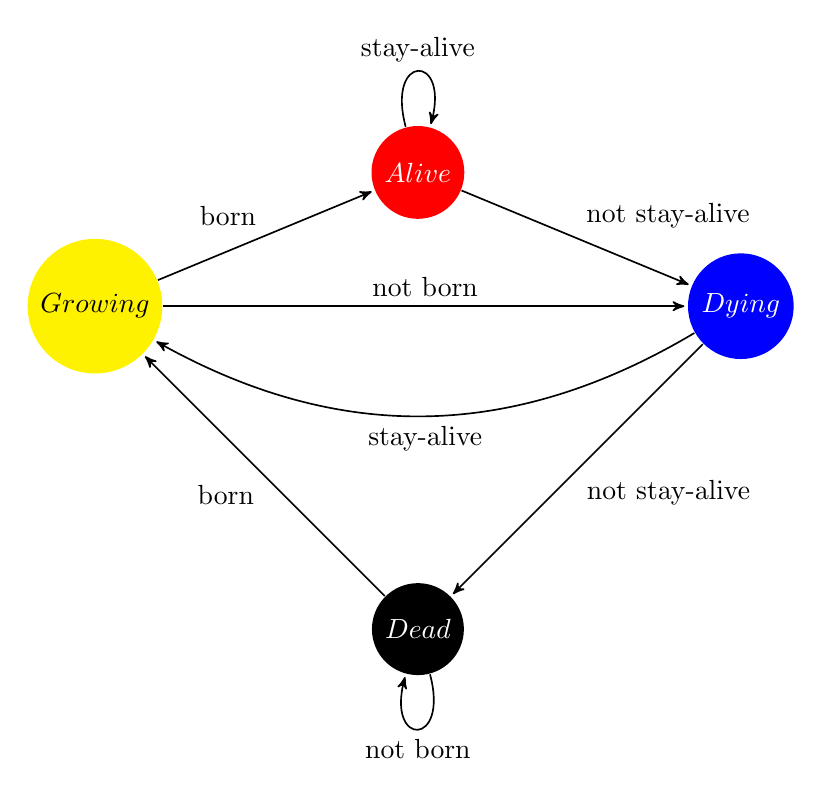
\begin{tikzpicture}[->,>=stealth',shorten >=1pt,auto,node distance=5.8cm,
                    semithick]
  \tikzstyle{every state}=[fill=red,draw=none,text=white]

  \node[state] (Dead)        [fill=black]            {$Dead$};
  \node[state]         (Growing) [above left of=Dead, fill=yellow, text=black] {$Growing$};
  \node[state]         (Alive) [above of=Dead, fill=red] {$Alive$};
  \node[state]         (Dying) [above right of=Dead, fill=blue] {$Dying$};

  \path (Dead) edge  [loop below]  node {not born} (Dead)
            edge              node {born} (Growing)
        (Growing) edge              node {born} (Alive)
            edge              node {not born} (Dying)
        (Alive) edge [loop above] node {stay-alive} (Alive)
            edge              node {not stay-alive} (Dying)
        (Dying) edge [bend left] node {stay-alive} (Growing)
            edge              node {not stay-alive} (Dead);
\end{tikzpicture}
\caption{\label{fig:statemachine}State transition of ruleset 2}
\end{figure}


\newpage
\section{Screenshot}
\begin{figure}[h!]
        \centering
        \begin{subfigure}[b]{0.5\textwidth}
                \includegraphics[width=\textwidth]{r2out}
                \caption{Stablized universe on ruleset 2}
                \label{fig:r2out}
        \end{subfigure}

        \caption{Stablized universe}
\end{figure}

\end{document}
